\documentclass[onecolumn,amsmath,amssymb,showpacs,prl,superscriptaddress,aps]{revtex4-1}

\usepackage{epsfig}
\usepackage{color}
\usepackage{array}
%\usepackage{subcaption}
\usepackage{graphicx}
\usepackage{bm}
\usepackage{epstopdf}


\DeclareMathOperator*{\argmin}{argmin}
\DeclareMathOperator\erf{erf}
\DeclareMathOperator\erfc{erfc}



\begin{document}

\title{Supplementary Material for ``Engineering momentum profiles of cold-atom beams"}

\author{D~Hudson \surname{Smith}}
\affiliation{Clemson University, Clemson, South Carolina 29634, USA}

\author{Artem~G \surname{Volosniev}}
\affiliation{Institut f{\"u}r Kernphysik, Technische Universit{\"a}t Darmstadt, 64289 Darmstadt, Germany}


\date{\today}

\maketitle

\section{Impurity in a Bose gas}


To model one impurity atom that moves through a one-dimensional environment made of $N$ cold bosonic atoms, we employ the following Hamiltonian
\begin{equation}
H=-\frac{\hbar^2}{2m}\sum_{i=1}^N\frac{\partial^2}{\partial x_i^2}-\frac{\hbar^2}{2M}\frac{\partial^2}{\partial y^2}+\lambda \sum_{i>j=1}^N\delta(x_i-x_j)+g \sum_{i=1}^N \delta(x_i-y),
\end{equation}
where $M$ is the mass of the impurity atom, and $m$ is the mass of a bosonic particle. The position of the impurity is $y$, bosons are at the coordinates $\{x_i\}$. 
We assume that the realistic boson-boson and boson-impurity interactions are well-described by the zero-range potentials of strengths $\lambda$ and $g$, respectively. 
The environment is large by assumption. To describe it, the periodic boundary conditions are used: The particles move in a ring of the circumference $L$, such that $0<x_i<L$ and $0<y<L$.
We are interested in the thermodynamic limit: $N, L\to \infty$ with a fixed value of the density $\rho=\frac{N}{L}$.


If the system is non-interacting ($\lambda=g=0$), the eigenstates are written as $e^{2\pi i \frac{n_1x_1+\ldots+n_N x_N+my}{L}}$, where $n_1,\ldots,n_N$ and $m$ are arbitrary integers. 
For non-vanishing interactions we use these functions to write an eigenfunction of the Hamiltonian as $\Psi=\sum_{\{n_j\},m} a_{\{n_j\},m}e^{2\pi i \frac{\sum n_jx_j+my}{L}}$. 
Because all interactions are pairwise, 
the total (angular) momentum of the system must be conserved, and we write it as ${\cal P}=\frac{2\pi\hbar}{L}\left(\sum_{j} n_j+m\right)$.
A conserved quantity (${\cal P}$) allows us to exclude one variable from the consideration. 
We write the function $\Psi$ as $\Psi=e^{i \frac{{\cal P} y}{\hbar}}\sum_{\{n_j\},m} a_{\{n_j\},m}e^{2\pi i \frac{\sum n_jz_j}{L}}\equiv e^{i \frac{{\cal P} y}{\hbar}} \psi(z_1,...,z_N)$ 
with $z_i=L\theta(y-x_i)+x_i-y$, where $\theta(x)$ is the Heaviside step function, i.e., 
$\theta(x>0) = 1$ and zero otherwise. The variables $z_i$ are defined such that $0\leq z_i \leq L$ and the impurity is placed at $z=0$ ($z=L$). Now if we insert this 
function into the Schr{\"o}dinger equation, $H\Psi=E\Psi$, we obtain the following equation for $\psi(0<z_i<L)$
\begin{equation}
-\frac{\hbar^2}{2m}\sum_i\frac{\partial^2 \psi}{\partial z_i^2}-\frac{\hbar^2}{2M}\left(\sum_{i}\frac{\partial }{\partial z_i}\right)^2\psi
+ i \frac{\hbar {\cal P}}{M}\sum_{i}\frac{\partial \psi}{\partial z_i}+\lambda \sum_{i>j}\delta(z_i-z_j)\psi=\left(E-\frac{{\cal P}^2}{2M}\right)\psi,
\end{equation}
which must be supplemented with the boundary conditions:
\begin{equation}
\psi(z_i=0)=\psi(z_i=L); \qquad \frac{\partial \psi}{\partial z_i}\bigg|^{z_i=0^+}_{z_i=L^-}= \frac{2 g \kappa}{\hbar^2} \psi(z_i=0),
\end{equation}
where $\kappa=mM/(m+M)$ is the reduced mass.

By assumption the bosons interact weakly, such that the ansatz $\psi=\prod_i \Phi(z_i)$ can be used to approximate the system. 
To minimize the expectation value of the Hamiltonian the function $\Phi(z)$ must satisfy the following non-linear Schr{\"o}dinger equation
\begin{equation}
-\frac{\hbar^2}{2\kappa}\frac{\partial^2\Phi}{\partial z^2}+i\frac{\hbar {\cal P}}{M}\frac{\partial \Phi}{\partial z}
-i \frac{\hbar^2 (N-1) A}{M} \frac{\partial\Phi}{\partial z} + \lambda (N-1)|\Phi|^2\Phi=\mu \Phi,
\end{equation}
where $A=-i\int \Phi(x)^*\frac{\partial}{\partial x}\Phi(x)\mathrm{d}x$ defines the momentum of a boson, and $\mu$ is the Lagrange multiplier. 
We rewrite this equation as
\begin{equation}
-\frac{\partial^2\Phi}{\partial z^2}+i v \frac{\partial \Phi}{\partial z} + \tilde \lambda (N-1)|\Phi|^2\Phi=\tilde\mu\Phi,
\label{eq:GPE_resc}
\end{equation}
where $\tilde\mu=\frac{2 \kappa \mu}{\hbar^2}$, $\tilde \lambda =\frac{2 \kappa \lambda}{\hbar^2}$, and 
$v= \frac{2 \kappa P}{M \hbar}$ with $P={\cal P}-\hbar A(N-1)$. $P$ defines the momentum of the impurity in the thermodynamic limit;
note that $A$ is determined by $P$, and there is a unique value of ${\cal P}$ for a given $P$.
The boundary conditions for Eq.~(\ref{eq:GPE_resc}) read
\begin{equation}
\Phi(z=0)=\Phi(z=L); \qquad \frac{\partial \Phi}{\partial z}\bigg|^{z=0^+}_{z=L^-}= \tilde g \Phi(0),
\end{equation}
where $\tilde g= \frac{2\kappa g}{\hbar^2}$. The non-linear equation~(\ref{eq:GPE_resc}) 
has an analytic steady solution~\cite{hakim1997}, which determines the properties 
of the dressed impurity in our problem. Let us first consider the non-interacting impurity $g=0$. 
In this case the solution for $v>0$ is~\cite{tsuzuki1971, ishikawa1980}
\begin{equation}
\Phi=\sqrt{\frac{\tilde \mu}{\tilde \lambda (N-1)}}\left(1-\beta \mathrm{sech}^2\left[\sqrt{\frac{\tilde\mu\beta}{2}}(z+z_0)\right]\right)^{\frac{1}{2}}e^{i\phi(z)},
\label{eq:Phi_c0}
\end{equation}
\begin{equation}
\phi(z)=-\pi\theta(z+z_d)+\mathrm{arctan}\left(\frac{\sqrt{\frac{2 v^2}{\tilde \mu}\beta}}{\mathrm{exp}\left[\sqrt{2\tilde \mu\beta}(z+z_0)\right]-2\beta+1}\right),
\label{eq:phi_c0}
\end{equation}
where  $\beta=1- v^2/(2\tilde \mu)$, $z_0$ is some parameter that determines the origin and $z_d$ is the point where $\mathrm{arctan}$ reaches $\pi/2$.
 It is worthwhile noting that the solution for $v<0$ is $\Phi^*$. 
The solution from Eqs.~(\ref{eq:Phi_c0}) and~(\ref{eq:phi_c0}) is plotted in Fig.~\ref{fig:Fig1}; 
for simplicity it is plotted in the interval $-L/2<z<L/2$, the region $0<z<L$ easily follows. 


%%%%%%%%%%%%%%%%%%%%%%%%%%%%%%%%%%%%%%%%%%%%%%%%%%%%%%%%%%%%%%%%%%%%%%%%%%%%%%%%%%%%%%%%%%%%%%%%%%%%%%%%%%%%%%%%%%%%%%%%
 \begin{figure}
 \centerline{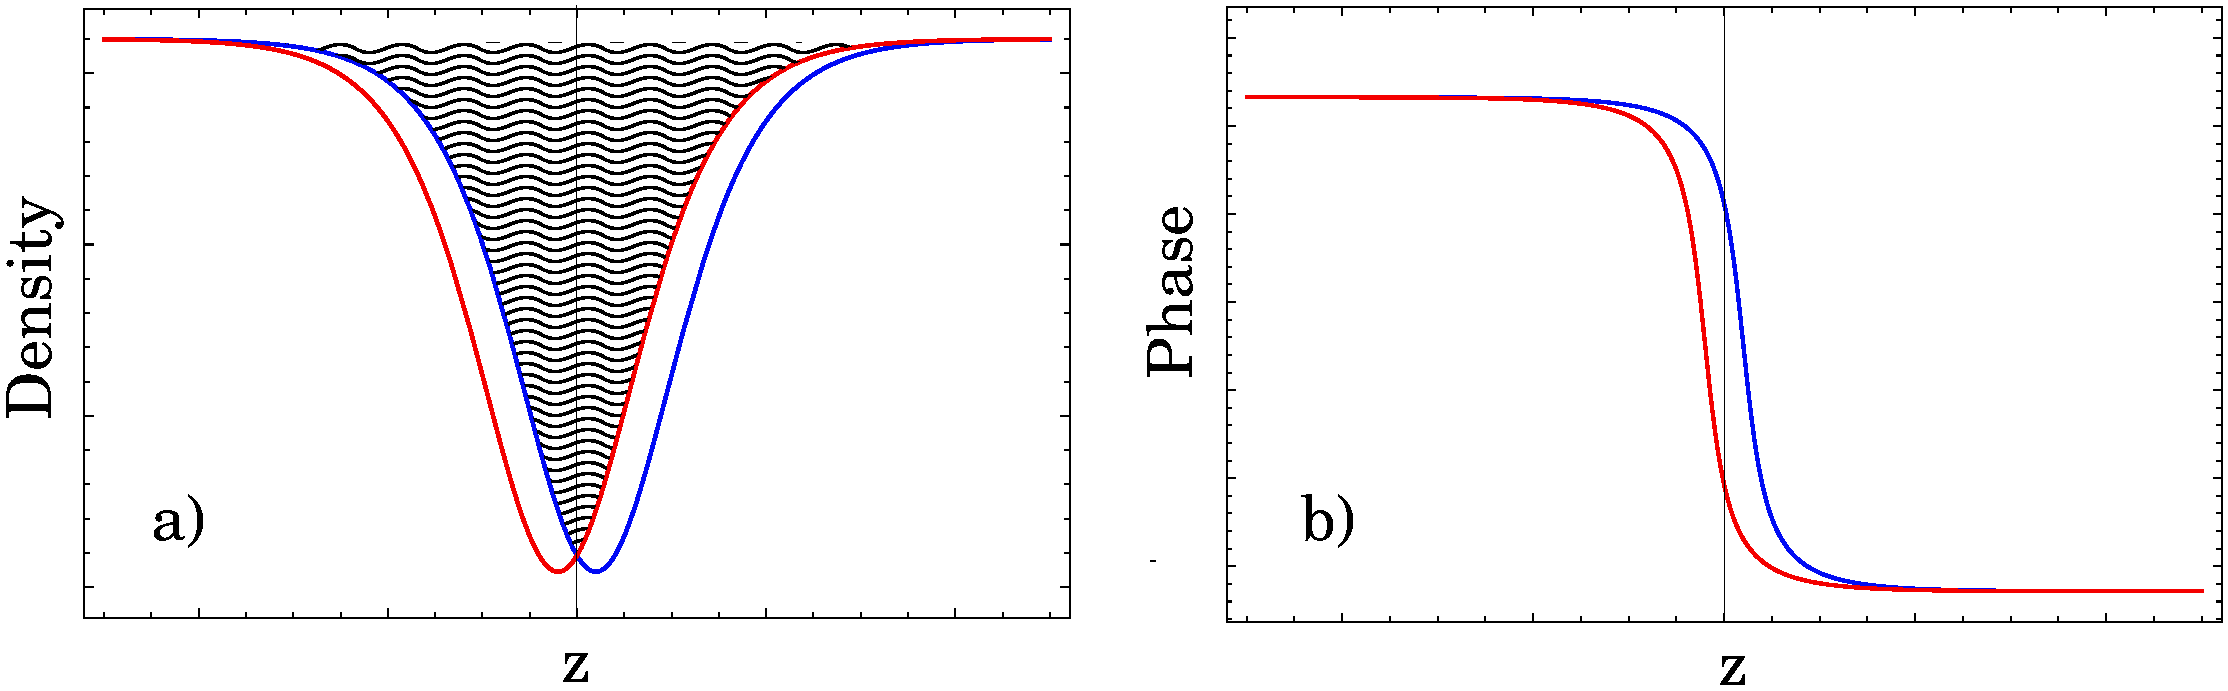
\includegraphics[scale=0.45]{figure1appendix_new.pdf}}
\caption{Panel {\bf a)}: The density, $|\Phi|^2 N$, of the Bose gas for $z_0=a$ (red curve), $z_0=-a$ (blue curve) 
($a>0$, the exact value of $a$ is not important for our discussion). 
 Note that the minimum of the density is at $-a$. 
The shaded area is a combination of the two solutions with the singularity at $z=0$. 
Panel {\bf b)}: The phase, $\phi$, of the Bose gas for the densities from {\bf a)}.}
 \label{fig:Fig1}
 \end{figure}
 %%%%%%%%%%%%%%%%%%%%%%%%%%%%%%%%%%%%%%%%%%%%%%%%%%%%%%%%%%%%%%%%%%%%%%%%%%%%%%%%%%%%%%%%%%%%%%%%%%%%%%%%%%%%%%%%%%%%%%%

To describe an interacting impurity, we combine two moving solitons with $\pm z_0$, which creates a singularity at $z=0$~\cite{hakim1997,kamenev2016}.
Therefore, a dressed impurity in our model is a topological defect with a dissipationless propagation. 
We write the corresponding `wave function' as
\begin{equation}
\Phi=\sqrt{\frac{\tilde \mu}{\tilde \lambda (N-1)}}\left(1-\beta \mathrm{sech}^2\left[\sqrt{\frac{\tilde\mu\beta}{2}}(z\pm z_0)\right]\right)^{\frac{1}{2}}e^{i\phi(z)},
\end{equation}
with 
\begin{equation}
\phi(z)=\delta \phi \theta(-z)+\mathrm{arctan}\left(\frac{\sqrt{\frac{2 v^2}{\tilde \mu}\beta}}{\mathrm{exp}\left[\sqrt{2\tilde \mu\beta}(z\pm z_0)\right]-2\beta+1}\right),
\label{eq:phase_soliton}
\end{equation}
where $z_0>0$ is discussed below, the parameter $\delta \phi$ is not important for the further derivations, it reassures that the phase is a continuous function;
the plus sign in $\pm$ corresponds to $z>0$ and the minus sign to $z<0$. This function is illustrated in Fig.~\ref{fig:Fig1}. 
The density has a non-analytic derivative at $z=0$. The phase is a continuous function at $z=0$ (its derivative is also continuous).
Note that the wave function is not periodic (see Eq.~(\ref{eq:phase_soliton})). This non-periodicity is not important 
for our discussion, because we are interested in the behavior of the bosons close to the impurity. It suggests that a grey soliton
must be formed upon a change of interaction parameters to take care of the phase slip.

The parameter $\tilde \mu$ is found from the normalization condition $\int \Phi^2=1$. For $N\to\infty$, we obtain
\begin{equation}
\tilde \mu=\gamma \rho^2 \frac{N-1}{N}\left(1-2\sqrt{2\beta_0} \frac{ (\mathrm{tanh}(d)-1)}{\sqrt{\gamma}N}\right),
\end{equation}
where $\gamma=\tilde \lambda /\rho$, $\rho=N/L$, $\beta_0=1-v^2/(2\gamma \rho^2)$, and $d=\sqrt{\frac{\gamma \beta_0}{2}}\rho z_0$.
The equation to determine $z_0$ is found by using the boundary conditions at $z=\{0,L\}$
\begin{equation}
\frac{\tilde g}{\rho \sqrt{2\gamma}}=\frac{\beta_0^{\frac{3}{2}}\tanh(d)}{-\beta_0+\cosh^2(d)}.
\label{eq:c_v}
\end{equation}
This equation is cubic (in $\tanh(d)$), hence, the solutions can be found in a closed form.
There are three solutions. However, only two will lead to the acceptable values of $z_0$. 
We will refer to these steady solutions as the `polaron' and the `polaron-soliton' pair, because in the limit $g\to 0$ the former 
corresponds to the ground state, and the latter to a gray soliton. 
The `polaron-soliton' pair is expected to be unstable (small perturbations lead to 
a decay of this steady solution~\cite{hakim1997}),
therefore, we do not consider it. The solutions merge for $z_m$ 
\begin{equation}
\tanh^2\left(\sqrt{\frac{\gamma \beta_0}{2}}\rho z_m\right)=\frac{\sqrt{1+\frac{4v^2}{\gamma \rho^2}}-(1+\frac{v^2}{\gamma \rho^2})}{2\beta_0},
\label{eq:z_m}
\end{equation}
which is derived by taking a derivative of Eq.~(\ref{eq:c_v}) with respect to $z_0$ and equating the resulting expression to zero -- this determines 
the maximum value of $g$ for which (for a fixed $\beta_0$) there is a steady solution.
Equations~(\ref{eq:c_v}) and (\ref{eq:z_m}) give the equation for the critical value of $v_c$:
\begin{equation}
\frac{\tilde g}{\rho\sqrt{\gamma}}=\frac{3-\sqrt{1+\frac{4v_c^2}{\gamma \rho^2}}}{-1+\sqrt{1+\frac{4v_c^2}{\gamma \rho^2}}}\sqrt{\sqrt{1+\frac{4v_c^2}{\gamma \rho}}-1-\frac{v_c^2}{\gamma\rho^2}}.
\end{equation}
For $v>v_c$ (see Fig. 4 of the main text) there is no steady solutions.


Now we can calculate the energy of the dressed impurity in the thermodynamic limit
\begin{equation}
{\cal E}\equiv \lim_{N\to\infty, \frac{N}{L}\to \rho}\left[E(c,P)-E(c=0,P=0)\right],
\end{equation}
where
\begin{equation}
E(c,P) = \frac{{\mathcal P}^2}{2M} + \mu N-\frac{\hbar^2 A^2 N(N-1)}{2M}-\lambda N(N-1)\int_{0}^{L/2}|\Phi|^4\mathrm{d}z.
\end{equation}
Using these expressions we derive 
\begin{equation}
{\cal E}=\frac{P^2}{2M}+\frac{\hbar^2\rho^2}{2\kappa}\frac{\sqrt{2  \gamma \beta}}{3}\left[4 b + (-4b+\beta\mathrm{sech}^2(d))\tanh(d)\right]+\frac{\hbar P}{M}\lim_{N\to\infty} A N,
\end{equation}
where $b=1+\frac{v^2}{4\tilde \lambda \rho}=1+\frac{\kappa P^2}{2M^2 \lambda \rho}$. This energy for $v\to 0$ can be written as 
\begin{equation}
{\cal E}\simeq \epsilon+ \frac{P^2}{2m_{\mathrm{\mathrm{eff}}}},
\label{eq:18}
\end{equation}
where $\epsilon$ is the effective energy of the dressed impurity, and $m_{\mathrm{eff}}$ is the effective mass.

The parameters $m_{\mathrm{eff}}$ and $\epsilon$ calculated using Eq.~(\ref{eq:18})  
agree well with the results in the literature~\cite{mistakidis2018}, supporting 
the use of the non-linear Schr{\"o}dinger equation for solving the problem. 
However, further work is required to understand other properties of a dressed impurity in this formalism.
First of all, it will be interesting to investigate the critical momentum,
which is supersonic in the employed model for $g\to 0$ and for not heavy impurities.
Indeed, the model we solve is equivalent to a heavy impurity moving in a gas of bosons with mass $\kappa$,  
which has a different speed of sound. 
Note that Fig.~4 of the main text reports on a heavy impurity ($M/m\gg 1$) for which this problem does not occur.
It will be also interesting to investigate the residue -- the overlap between the wave function that describes 
a state with $g=0$ and the wave function that decribes an interacting state. In the present model, the impurity changes the order parameter
only locally, which means a non-zero residue (see~\cite{volosniev2017} for $P=0$), contradicting other 
studies on the topic~\cite{pastukhov2017,grusdt2017}. To understand this disagreement, one could calculate the overlap using an exactly solvable model, e.g., 
a heavy impenetrable impurity in a Bose gas (solvable by Bethe ansatz). 


\section{Boundary-Augmented Cost Function}\label{sec:Jaug}
Equation~(6) shows the boundary-augmented cost function which includes a term that increases the cost for link-potential solutions that extend beyond the support region $x\in[-x_0,x_0]$. This added terms is
\begin{equation}
  J_{\mathrm{boundary}} = \alpha \sum_i^N J_{\mathrm{boundary}}^i,
\end{equation}
where 
\begin{equation}\label{eq:Jboundaryi}
  J_{\mathrm{boundary}}^i = \int\limits_{|x|>x_0}dx\,|V_i(x; A_i,\mu_i,\sigma_i)|^2.
\end{equation}
Assuming the Gaussian potential form as in Eq.~(5), this evaluates to
\begin{equation}\label{eq:JboundaryIGaussian}
  J_{\mathrm{boundary}}^i = \frac{\sqrt{\pi}}{2}A_i^2\sigma_i\left[
    \erfc\left(\frac{x_0+\mu_i}{\sigma_i}\right) +
    \erfc\left(\frac{x_0-\mu_i}{\sigma_i}\right)
  \right],
\end{equation}
where $\erfc$ is the complementary error function.


\bibliographystyle{apsrev4-1}
\bibliography{bib}

 \end{document}


